\documentclass[10pt, a4paper]{article}
\usepackage[utf8]{inputenc}
\usepackage{pdflscape}
\usepackage{amssymb}
% \usepackage[margin=3cm]{geometry}
\usepackage{graphicx}
\usepackage{oz}
\usepackage{array,multirow,makecell}
\setcellgapes{1pt}
\usepackage[top=4cm,bottom=4cm,left=3cm,right=3cm]{geometry} %marges
\newcolumntype{R}[1]{>{\raggedleft\arraybackslash }b{#1}}
\newcolumntype{L}[1]{>{\raggedright\arraybackslash }b{#1}}
\newcolumntype{C}[1]{>{\centering\arraybackslash }b{#1}}

\title{Analyse Projet BDD}
\date{}
\begin{document}


\maketitle
\tableofcontents
\newpage

\section{Analyse du problème}
\subsection{Hypothèses}
Pour la conception, nous avons fait les choix suivants:
\begin{enumerate}
    \item Le statut des commandes n'est pas dans l'entité mère COMMANDES 
mais dans ses sous-entités afin d'éviter d'avoir des statuts non cohérents 
pour un type de commande donné.
    \item Nous avons rajouté le statut ``terminée'' qui indique qu'une 
commande a effectivement été effectuée et que l'on peut donner un 
évaluation
    \item Nous avons choisi, lorsque le client fait appel au droit à l'oubli de ne pas lui créer de nouvel identifiant car il en possède déjà
    un qui est uniquement vu par la base de données et auquel il n'a pas accès. Cette modification n'aurait donc était qu'une modification de nombreuses tables.
    \item Concernant les statuts des commandes, nous supposerons que ce sont les restaurants qui s'soccuperont d'actualiser dans la base de données leur commande.
    \item pour les catégories, nous avons ajouté une catégorie mère '\_' qui est la racine des catégories.
    Ainsi, chaque restaurant a une catégorie qui est au pire, la catégorie '\_'.
\end{enumerate}

Nous sommes arrivés avec les contraintes suivantes :
\begin{landscape}
\subsection{Contraintes}

\begin{center}
\[
\begin{tabular}{|C{5cm}|C{5cm}|C{5cm}|C{5cm} |}

\hline
DF& C. Valeurs 
& C. Contextuelles & C. Multiplicité\\
\hline

RMail $\rightarrow$ RNom, RNumero, RAdresse, Places, 
Presentation, RNote & RType $\in$ \{livraison, emporter, place\} & $\sum 
\mbox{nbPers}  \le \mbox{Places} $ pour un restaurant et ses commandes 
associées & RMail $\twoheadrightarrow$ JourPlage\\

 & Places $> 0$ & $\mbox{Ext(CEId)} \cap \mbox{Ext(CPId)} \cap 
\mbox{Ext(CLId)} = \emptyset $ &  RMail  $\twoheadrightarrow$ 
TypeCommande\\ 
 
 & RNote $\in  [0,5] $ &  $\mbox{Ext(CEId)} \cup \mbox{Ext(CPId)} \cup 
\mbox{Ext(CLId)} = \mbox{Ext(CId)}$ & RMail $\twoheadrightarrow$ PId\\
\cline{1-2}

(PId, Restaurant) $\rightarrow$ PNom, PDescription, PPrix & PPrix $>0$ & 
CPArrivee $\in$ JourPlage pour un restaurant et ses commandes associées & 
RMail $\twoheadrightarrow$ CatNom\\
\cline{1-2}

U\_Id $\rightarrow$ UMail, UMdp, UNom, UPrenom, UAdresse && CDate donne JourPlage pour toute commande& (PId, RMail) $\psur$ ANom \\
\cline{1-2}

CId $\rightarrow$ CDate, CPrix & CPrix $>0$ & CDate $\le$ EDate& 
CId $\twoheadrightarrow$ (PId, RMail)\\
\cline{1-2}

CLId $\rightarrow$ CLAdresse, Indications, CLArrivee, CLStatut & 
CLStatut $\in$ \{ attente, validée, en livraison, annuleeC, annuleeR, 
terminee \}&
EId $\Rightarrow$ CId.statut = \{terminee\}
& CId $\rightarrow$ TypeCommande \\ 
\cline{1-2}

CEId $\rightarrow$ CEStatut &
CEStatut $\in$ \{ attente, validée, disponible, annuleeC, annuleeR, terminee \}&  & CId $\rightarrow$ U\_Id\\
\cline{1-2}

CPId $\rightarrow$ NbPers, CPArrivee, CPStatut &
CPStatut $\in$ \{ attente, validée, annuleeC, annuleeR, 
terminee \}&  & CId $\pfun$ 
EId\\

& NbPers $>0$ & & CatNom $\pfun$ CatNom\\
\cline{1-2}

EId $ \rightarrow$ EDate, Avis, ENote & ENote $ \in [0..5] $&
CType $\in$ TypeCommande pour un CId donné et le RMail associé &\\ 
\cline{1-2}

& JourHeure $\in $ \{LM, LS, MaM, MaS, MeM, MeS, JM, JS, VM, VS, SM, SS, DM, 
DS \} & & \\
\hline

\end{tabular}
\]
\end{center}


\newpage
\subsection{Diagramme Entités/Associations}
On obtient ensuite le diagramme Entité-Relation suivant:
\begin{center}
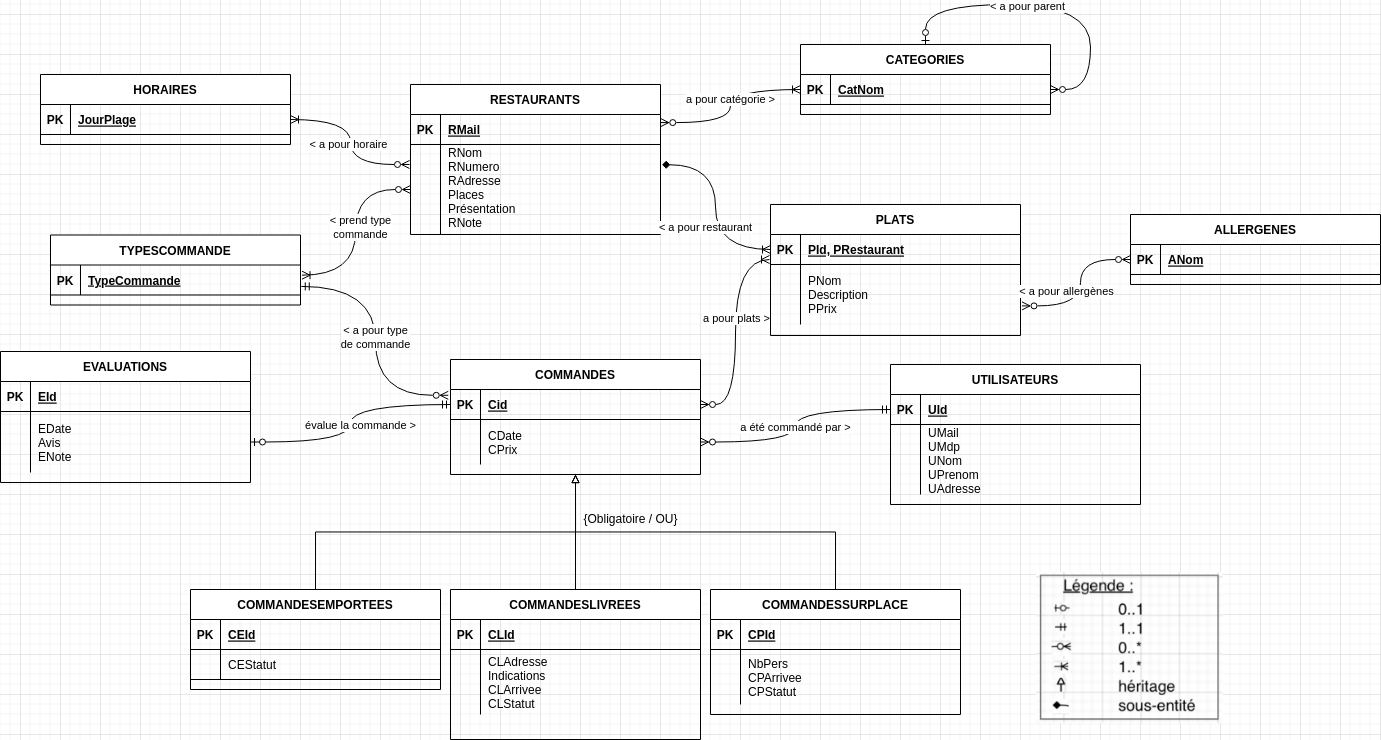
\includegraphics[scale=0.7]{Diagramme_entite_relation.png}\\
\end{center}

\end{landscape}
\section{Modèle Relationnel}

Nous avons appliqué l'algorithme vu en cours pour obtenir le schéma relationnel.

\subsection{Traduction des entités simples}

Nous avons identifié les entités simples suivantes:

\begin{itemize}
    \item Restaurant\@(\underline{RMail}, RNom, RNum, RAdresse, Places, Présentation, RNote)
    \item Commandes\@(\underline{Cid}, CDate, CPrix, \textbf{Uid}, \textbf{TypeCommande})
    \item Utilisateurs\@(\underline{U\_id}, UMail, UMdp, UNom, UPrenom, UAdresse)
    \item Evaluation\@(\underline{Eid}, EDate, Avis, ENote, \textbf{Cid})
    \item Horaires\@(\underline{JourPlage})
    \item TypesCommande\@(\underline{TypeCommande})
    \item Categories\@(\underline{CatNom})
    \item Allergenes\@(\underline{ANom})
\end{itemize}

\subsection{Sous-types d'entités}

Pour une question d'espace occupé nous avons décidé de traduire l'héritage des différentes catégories des commandes par référence. 
Contrairement à l'unification cela nous permet de ne pas avoir à gérer les contraintes avec l'application.

\begin{itemize}
    \item CommandesEmportees\@(\underline{CEid}, CEStatut)
    \item CommandesLivrees\@(\underline{CLid}, CLAdresse, Indications, CLArrivee, CLStatut)
    \item CommandesSurPlace\@(\underline{CPid}, NbPers, CPArrivee, CPStatut)
\end{itemize}

\subsection{Type d'entité faible}

\begin{itemize}
    \item Plats\@(Pid, PRestaurant, PNom, Description, PPrix)
\end{itemize}

\textbf{Contrainte induite par la traduction}: Vérifier que tout restaurant a au moins un plat.

\subsection{Types d'associations}

\subsubsection{Cardinalité 1..1}

Les attributs en gras dans les relations de la partie 2.1 correspondent aux traductions des associations avec cardinalité 1..1. 
Aucune vérification supplémentaire n'est à faire.
\subsubsection{Cardinalité 0..1}

\begin{itemize}
    \item CategorieParent\@(\underline{CatNom, CatNomMere})
\end{itemize}

\subsubsection{Cardinalité ?..*}

\begin{itemize}
    \item HorairesRestaurant\@(\underline{RMail, JourPlage})\\
    \textbf{Contrainte induite}: Vérifier qu'un restaurant a au moins un horaire.
    \item CategoriesRestaurant\@(\underline{RMail, CatNom})\\
    \textbf{Contrainte induite}: Vérifier qu'un restaurant a au moins une catégorie
    \item TypesRestaurant\@(\underline{RMail, TypeCommande})\\
    \textbf{Contrainte induite}: Vérifier qu'un restaurant a au moins un type de commande.
    \item PlatsCommande\@(\underline{Cid, Pid, PRestaurant})\\
    \textbf{Contrainte induite}: Vérifier qu'une commande a au moins un plat.
    \item AllergenesPlat\@(\underline{Pid, PRestaurant, ANom})
\end{itemize}


\section{Analyse des fonctionnalités}
\subsection{Parcours des restaurants}
Pour obtenir la fiche de présentation des restaurants pour une catégorie donnée $categorie$ :
$$
\pi_{attr}(\sigma_{CatNom = 'categorie'}(CATEGORIESRESTAURANT \Join RESTAURANTS))
$$
Avec $attr = \left\{ RMail, RNom, Presentation, RNum, RAdresse, Place, Note \right\}$

\subsection{Droit à l'oubli}
Le droit à l'oubli modifie uniquement la table utilisateur mais n'est pas exprimable
avec l'algèbre relationnel.

\subsection{Passage de commande}
Pour le passage de la commande, il y a plusieurs requêtes nécessaires.
Les premières étapes :
\begin{itemize}
    \item Insertion de la commande
    \item Ajout des plats
    \item Ajout du type de la commande
\end{itemize}
ne seront pas exprimables avec l'algèbre relationnel car il s'agit de modifier les tables.
On peut toutefois récupérer les tuples (PPrix, NbPlats) qui vont servir à calculer le coût total pour une commande de Cid = $Cid_0$:
$$
\pi_{PPrix, NbPlats}( \sigma_{Cid = Cid_0}(PLATS \Join PLATSCOMMANDE))
$$
De même, il est possible d'avoir le nombre de personnes sur place pour toutes les commandes sur place passées pour un horaire demandé = $time$ et un restaurant = $restaurant$ :
$$
\pi_{Cid, NbPers}(\sigma_{CPArrivee - time < '4h'}(COMMANDES \Join_{CType = 'sur place'} COMMANDESSURPLACE 
$$
$$
\Join_{PRestaurant = 'restaurant'} PLATSCOMMANDE))
$$
On remarquera que dès que plusieurs plats auront été commandés pour une même commande, on aura alors
une répétition qu'i faudra donc trier avec l'API.

\section{Bilan du projet}
\subsection{Logan - gestion BD}
En commençant le projet j'étais enthousiaste d'avoir un projet mêlant différentes 
technologies afin de d'avoir en résultat un produit beaucoup plus concret. Je me suis dès le 
début occupé de la partie SQL avec l'analyse et la conception de la base de données. Cela m'a 
permis de réellement comprendre la méthode vue en cours, et ce, de manière bien plus efficace 
que lors des TDs.\\

En terme de difficultés relevées réside surtout les choix de conception, que ce soit dû à une
ambiguïté du sujet, ou bien seulement un manque d'informations. Savoir si le choix que l'on fait
s'avérera être utile ou handicapant pour la suite est une chose qui m'est souvent difficile de
faire. Une autre difficulté de trouve être l'analyse même de la base de données. Beaucoup 
d'informations sont présentes, on ne doit rien omettre et une erreur, ou un oubli, dès cette 
étape peut générer des problèmes ou des incohérences dans tout le projet.

En ce qui concerne les facilités, je pourrais citer l'étape de création du diagramme 
entités/associations ou encore le passage en relationnel. Puis plus généralement les requêtes 
SQL n'étaient pas un majeur problème que ce soit pour la création des tables, pour le 
peuplement ou les différents scripts SQL.\\

Enfin, je ne ferai pas tout un paragraphe sur la panne informatique, mais le seul regret que 
j'ai c'est d'avoir dû abandonner l'idée d'avoir un rendu de projet pleinement fonctionnel et 
concret puisque désormais il ne s'agit de ne discuter qu'autour de notre travail sur la base de
donnée sans pouvoir s'appuyer sur un démonstrateur.
Pour conclure avec mon appréciation générale, je dirais que c'était pour moi un projet 
intéressant, la répartition du travail était claire et plutôt efficace et l'ambiance de groupe 
l'était tout autant.

\subsection{Maud - gestion BD}
Pour ma part, au début du projet j'avais peur de la quantité de travail à faire mais j'étais
en même temps très enthousiaste à l'idée d'implémenter une application et de voir l'interraction
application-base de données. Je me suis principalement focalisée sur l'analyse et la mise en 
place de la base de données.\\

Les difficultés éprouvées provenaient principalement de zones floues liées à l'énoncé et donc
des incertitudes sur la mise en place du schéma. En particulier, l'hérédité des catégories a été
compliquée à concevoir mais nous avons réussi à la mettre en place sans problème une fois La
solution trouvée.

La partie plus facile a été le remplissage des tables car bien qu'il ait été long, il ne
présentatit aucune difficulté. L'analyse en elle-même a été faite relativement facilement
ainsi que l'écriture des requêtes SQL.\\

Enfin, ce projet m'a beaucoup appris sur la conception de base de données. De même, j'ai trouvé
que l'ambiance était bonne et l'organisation du groupe a été efficace. Toutefois, je reste déçue
quant à la suppression de l'API de l'évaluation car dasn notre cas elle est fonctionnelle et terminée.

\subsection{Jorge - gestion API}
Les difficultés auxquelles j'ai fait face étaient les suivantes : tout d'abord la connexion entre la base de données
et l'API pour la première fois était compliquée à comprendre, difficulté qui s'est représentée
à la fin du projet lorsque nous avons utilisé SQLLite pour poursuivre notre projet. Ensuite,
l'envoi des commandes vers la base de données une fois que l'utilisateur avait fini sa commande 
a été compliqué à réaliser ainsi que d'implémenter les contraintes contextuelles car je 
n'avais que peu travaillé sur la partie relationnelle. \\

Toutefois, certains aspects ont été beaucoup plus simples que prévus, notamment le droit à l'oubli,
le parcours des catégories, la connexion/déconnexion de l'API par un utilisateur et l'écriture
des requêtes SQL pour les envoyer à la base de données.\\

Je me suis également occupé de l'interface utilisateur avec les différents menus ainsi que l'affichage
de 10 restaurants par 10 restaurants. Ces derniers aspects m'ont pris beaucoup de temps car
l'implémentation est longue bien que pas très complexe.


\section{Mode d'emploi}

Nous avons développé, comme demandé initialement, un démonstrateur en Java.

Après la panne informatique de l'Ensimag et la non-nécessité du démonstrateur, nous avons tout de même voulu 
rendre un démonstrateur fonctionnel, même si toutes les fonctionnalités n'ont pas été introduites. Ainsi, Oracle n'étant pas accessible, 
nous avons développé la base de données en SQLite, en local.

Nous avons alors exporté le démonstrateur dans un \texttt{.jar}. Pour démarrer le démonstrateur, il faut aller 
dans le dossier Interpréteur et lancer la commande \texttt{java -jar GrenobleEAT.jar}. \\


La navigation dans le navigateur est assez intuitive. L'utilisateur peut naviguer de menu en menu en suivant 
les instructions demandées. Pour sélectionner les options proposées par  démonstrateur, l'utilisateur devra 
introduire soit le chiffre correspondant à l'option souhaitée, soit exactement écrire l'option souhaitée.
L'application indiquera quand est-ce qu'il faut introduire l'option en chiffre et quand il faudra le faire en toutes lettres. \\

Lorsqu'un utilisateur veut réaliser une commande, il peut soit voir la liste des restaurants soit explorer les catégories de l'application.

La liste des restaurants s'affiche dans l'ordre décroissant des évaluations des utilisateurs et dans l'ordre alphabétique des noms. \\

Pour l'exploration des catégories, tout d'abord l'application recommande à l'utilisateur les 3 dernières catégories
commandées. Puis, si les catégories ne conviennent pas à l'utilisateur ou si simplement l'utilisateur manque de commandes 
réalisées, nous avons choisi de faire un parcours sous forme d'arbre. Au début, l'application propose des catégories générales, et 
l'utilisateur peut soit sélectionner la catégorie courante, soit continuer à parcourir les sous-catégories. Puis, l'application montre 
les restaurants spécialisés dans les catégories choisies. \\

L'utilisateur peut alors choisir les plats qu'il veut dans le restaurant choisi. Une fois qu'il a fini sa sélection, l'utilisateur 
choisi entre commander en livraison, sur place ou à emporter. L'application demandera alors les informations complémentaires. \\

Pour s'identifier dans l'application, l'utilisateur doit soit indiquer son email et son mot de passe, soit créer un nouveau 
compte en introduisant toutes les données nécessaires. Si un utilisateur souhaite demander un effacement de ses données,
il est possible de le demander à l'application avec l'option correspondante via la page d'accueil. L'application efface 
alors toutes les données personnelles, tout en gardant l'identifiant unique de compte (U\_id). Ceci permet de garder les évaluations 
et l'historique des commandes sans que celles-ci soient attribuées à une nouvelle entrée des utilisateurs. \\

Finalement, l'utilisateur peut aussi évaluer les commandes réalisées dans le passé. Il pourra voir les commandes réalisées 
et choisir une note de 0 à 5, ainsi que laisser un commentaire optionnel.
\end{document}


